\section{Auswertung}
\subsection{Winkelabhängigkeit}
In diesem Versuch soll überprüft werden, ob die umhüllte Bauweise des Pitotrohrs tatsächlich die Winkelabhängigkeit des Messergebnisses reduziert.
Hierzu wurde das Pitotrohr, ähnlich wie bei der Messung auf dem Auto, zusammen mit der Prandtlsonde aus dem Lager als statischer Druckmesser in den Luftstrom einer Turbine gebracht. Der Winkel des Pitotrohrs gegenüber der Strömungsrichtung wurde verändert und der resultierende Druck wurde vom Feinmanometer abgelesen. Diese Messung wurde für drei verschiedene Strömungsgeschwindigkeiten, die mit einem Windmesser bestimmt wurden, durchgeführt. Als Messfehler wurde ein Ablesefehler von $\pm2$ Pa angesetzt.
\begin{figure}
        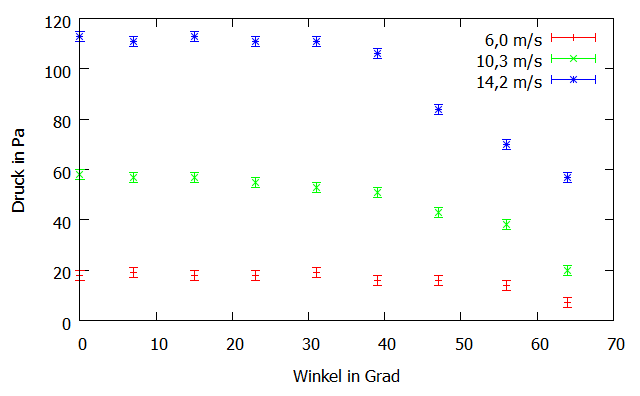
\includegraphics[width=.9\textwidth]{images/Winkel}
\caption{Messung der Winkelabhängigkeit des Pitotrohrs für 3 verschiedene Strömungsgeschwindigkeiten}
\label{fig:Winkel}
\end{figure}

Man sieht (Abbildung \ref{fig:Winkel}), dass im Rahmen des Messfehlers im Winkelbereich bis $30^\circ$ keine Abweichung festzustellen ist. Weiterhin fällt der Druck bei der Geschwindigkeit $14.2 \frac{m}{s}$ stärker ab als bei den kleineren Geschwindigkeiten, was aus der Theorie zu erwarten ist.
\\
Zum Vergleich soll noch die Winkelabhängigkeit der nicht umhüllten Prandtlsonde aus dem Lager überprüft werden. Dazu wurde der gleiche Versuchsaufbau wie vorher mit der Strömungsgeschwindigkeit $10.3 \frac{m}{s}$ verwendet. Es wurde wieder ein Ablesefehler von $\pm 2$ Pa angesetzt.
\begin{figure}
      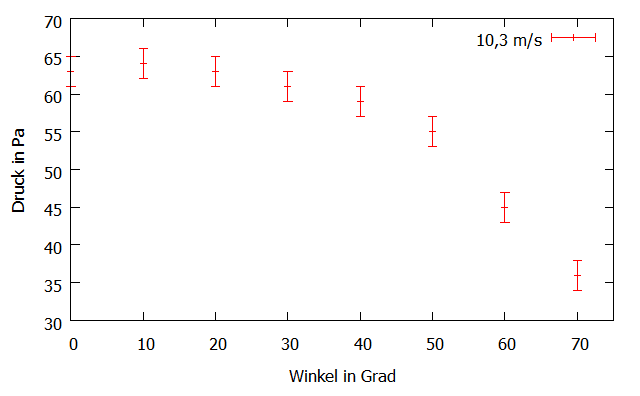
\includegraphics[width=.9\textwidth]{images/Winkelnormalrohr}
\caption{Messung der Winkelabhängigkeit der nicht umhüllten Prandtlsonde für eine Strömungsgeschwindigkeit von $10,3 \frac{m}{s}$}
\label{fig:Winkelnormalrohr}
\end{figure}
Auch hier (Abbildung \ref{fig:Winkelnormalrohr}) ist im Winkelbereich bis $30^\circ$ keine Abweichung festzustellen, obwohl das Rohr nicht umhüllt ist.
Es scheint also, als ob die umhüllte Bauweise des 3D-gedruckten Pitotrohrs keinen Unterschied machen würde. Jedoch ist der in der Theorie erwähnte Vorteil des umhüllten Pitotrohrs, dass der Fehler für einen bestimmten Winkelbereich unter $1\%$ liegt, mit unserer Messgenauigkeit unmöglich nachzuvollziehen. Das gewünschte Resultat für die Messung auf dem Auto, also dass das Messergebnis nicht stark vom Winkel beeinflusst wird, wurde aber erreicht.
\subsection{Kalibration des Rohrs}
Als Nächstes soll überprüft werden, ob das 3D-gedruckte Rohr korrekte Messergebnisse liefert und eine eventuelle Abweichung bestimmt werden.
\
Hierfür wurde das Pitotrohr wieder zusammen mit der Prandtlsonde als statischer Druckmesser in den Luftstrom einer Turbine gebracht. An der Turbine wurden verschiedene Geschwindigkeiten eingestellt, die mit einem Windmesser gemessen wurden, der resultierende Druck wurde am Feinmanometer abgelesen. Es wurde wieder ein Ablesefehler von $\pm 2 Pa$ angesetzt. Die gemessenen Drücke wurden mit der Bernoulli-Gleichung über Gleichung(\ref{eq:Geschwindigkeitsformel}) in Geschwindigkeiten umgerechnet.
Der Fehler für die Geschwindigkeiten wurde über Fehlerfortpflanzung mittels der Formel
\begin{equation}
\Delta u=\sqrt{(\frac{\partial u}{\partial p_D}\Delta p_D)^2}=\sqrt{(\frac{\Delta p_d}{\sqrt{2\rho p_D}})^2}
\label{eq:Fehlerfortpflanzung}
\end{equation}
bestimmt.
\begin{figure}
      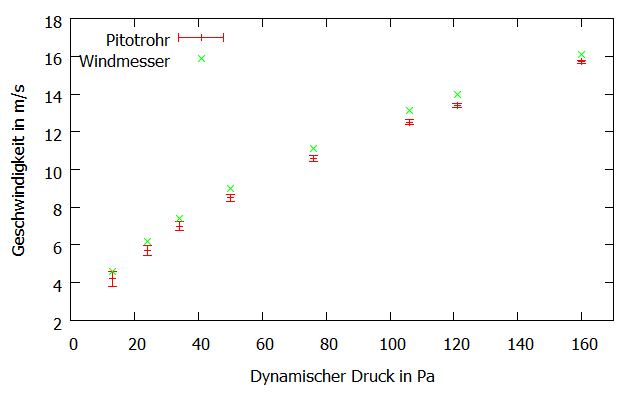
\includegraphics[width=.9\textwidth]{images/Kalibration}
\caption{Kalibration des Rohrs}
\label{fig:Kalibration}
\end{figure}
Die Ergebnisse sind in Abbildung \ref{fig:Kalibration} dargestellt. Die Werte auf der x-Achse sind hier die mit dem Windmesser gemessenen Geschwindigkeiten umgerechnet in Drücke. Aus der Grafik und den Messwerten (Tabelle \ref{tab:Kalibration2}, Seite \pageref{tab:Kalibration2} sieht man, dass sich die Abweichung (innerhalb des Messbereichs) nicht mit der Geschwindigkeit ändert. Deswegen kann nun eine mittlere Abweichung bestimmt werden. Eigentlich müsste hier der Fehler aus der Fehlerfortpflanzung mit eingerechnet werden, dies wäre aber sehr kompliziert und muss deshalb vernachlässigt werden. Die mittlere Abweichung ergibt sich dann (mit statistischem Fehler) zu:
\begin{equation}
\Delta u= 0,49 \pm 0,03 \frac{m}{s}
\label{eq:Abweichung}
\end{equation}
Der Grund für diese Abweichung kann nicht klar bestimmt werden, es ist aber anzunehmen, dass Fehler und Ungenauigkeiten beim 3D-Druckprozess (z.B. rauhe Oberflächen, kleine Verformungen des Materials, etc.) zumindest teilweise dafür verantwortlich sind.
\subsection{Geschwindigkeitsmessung}
Für die Auswertung der Geschwindigkeitsmessung wurden die Videoaufnahmen des Tachometers mit denen des Manometers synchronisiert. Dazu wurde die Audiospur der beiden Kameras durch die Software Pluraleyes analysiert, welche eine XML Datei zum Import in gängige Videoschnittprogramme erstellt. Es stellte sich jedoch heraus, dass die Audiospuren keine gute Qualität aufwiesen. Dies führte zu einer fehlerbehafteten Synchronisation, sodass teilweise Abweichungen von mehreren Sekunden zwischen beiden Videos vorkommen.
Aus dem synchronisierten Video wurden dann die Passagen, während denen mit konstanter Geschwindigkeit gefahren wurde, herausgesucht. Aus diesen Passagen wurden dann jeweils ein Startpunkt, an dem die Flüssigkeit im Manometer nicht mehr steigt bzw. fällt, und ein Endpunkt, an dem die Flüssigkeit wieder steigt bzw. fällt, d.h. wenn das Auto wieder beschleunigte bzw. abbremste, gewählt. Das Zeitintervall zwischen Start- und Endpunkt wurde dann in 10 gleiche Teile unterteilt und jeweils am Beginn eines neuen Teils wurde der Wert für den gemessenen Druck auf dem Manometer und der Wert für die mit GPS gemessene Geschwindigkeit aufgeschrieben. (D.h. wenn z.B. ein 40 Sekunden langes Zeitintervall gewählt wurde, wurde alle 4 Sekunden ein Messwert aufgeschrieben.)
\\
Für das GPS wurde ein Fehler von $\pm 0,3$ Knoten gewählt, das dies der Wert war, der auch bei stehendem Fahrzeug angezeigt wurde. Für den Druck kann wieder ein Ablesefehler von $\pm 2$ Pa angenommen werden. Die gemessenen Drücke wurden dann über Gleichung (\ref{eq:Geschwindigkeitsformel}) in Geschwindigkeiten umgerechnet, aus denen dann ein Mittelwert und statistischer Fehler bestimmt wurde. Zu dem so bestimmten Mittelwert wurde dann noch die Abweichung (Gleichung (\ref{eq:Abweichung})) hinzuaddiert. Korrekterweise müsste hier wieder bei der Umrechnung der Drücke in Geschwindigkeiten eine Fehlerfortpflanzung nach Gleichung (\ref{eq:Fehlerfortpflanzung}) durchgeführt werden, die Behandlung dieser Fehler ist aber wieder sehr kompliziert und muss deswegen vernachlässigt werden. Für die mit GPS gemessenen Geschwindigkeiten wurden ebenfalls Mittelwerte und statistische Fehler bestimmt.
\\
\begin{figure}
      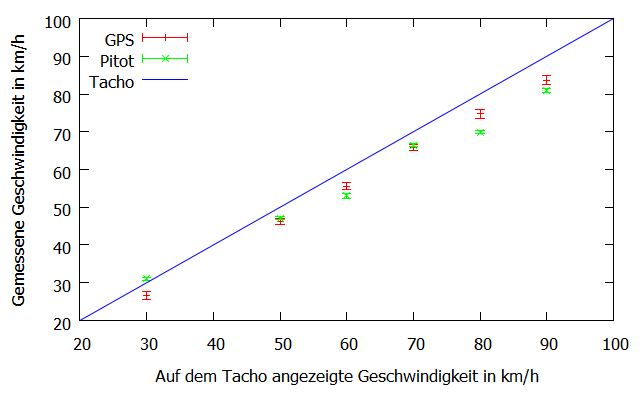
\includegraphics[width=.9\textwidth]{images/Geschwindigkeit}
\caption{Messung der Geschwindigkeit}
\label{fig:Geschwindigkeit}
\end{figure}
\\
Die Ergebnisse der Messung sind in Abbildung (\ref{fig:Geschwindigkeit}) dargestellt. Folgende Beobachtungen können gemacht werden:
\begin{enumerate}
\item Für 40 km/h ist kein Messwert eingetragen. Dies liegt daran, dass aufgrund der Verkehrslage nur kurzzeitig ($\backsim 20$ Sekunden) 40 km/h gefahren werden konnten. Wegen der fehlerhaften Synchronisation und der Verzögerung des Manometers können aus dem Video hierfür keine Messpunkte entnommen werden.
\item Der Fehler für die mit dem Pitotrohr bestimmten Werte ist zu klein, da die Fehler aus der Fehlerfortpflanzung notwendigerweise vernachlässigt wurden.
\item Die gemessenen Geschwindigkeiten sind größtenteils kleiner als die am Tachometer angezeigten. Dies soll im Folgenden noch näher untersucht werden.
\end{enumerate}
\begin{figure}
      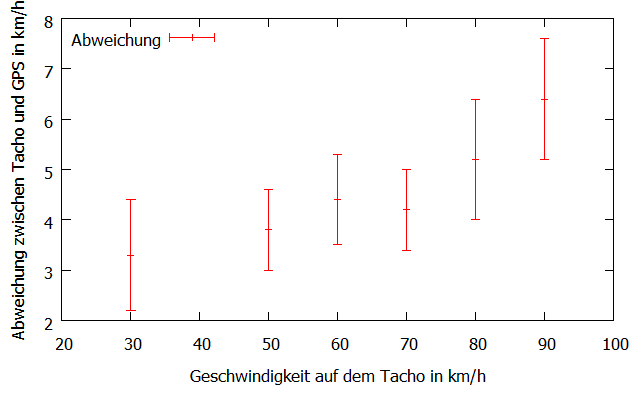
\includegraphics[width=.9\textwidth]{images/AbweichungGPSTacho}
\caption{Abweichung der am Tachometer angezeigten und mit GPS gemessenen Geschwindigkeit}
\label{fig:AbweichungGPSTacho}
\end{figure}
In Abbildung \ref{fig:AbweichungGPSTacho} ist die Differenz zwischen der am Tachometer angezeigten und mit GPS gemessenen Geschwindigkeit dargestellt. Es zeigt sich, dass die Abweichung relativ groß (im Bereich von 2-8 km/h) ist und mit der Geschwindigkeit zunimmt. Diese Abweichung liegt im Funktionsprinzip des Tachometers begründet. Tachometer messen die Drehzahl der Räder des Autos und errechnen daraus eine Geschwindigkeit. Zusätzlich zur prinzipiellen Ungenauigkeit der Messmethode verändern Abweichungen im Radumfang (z.B. durch Verschleiß oder Reifenwechsel) das Messergebnis. Diese Abweichungen wirken sich bei höheren Drehzahlen, d.h. höheren Geschwindigkeiten, stärker aus. Weiterhin ist gesetzlich vorgeschrieben, dass ein Tachometer aus Sicherheitsgründen niemals eine geringere Geschwindigkeit als die tatsächlich gefahrene anzeigen darf, weswegen Tachometer schon von Werk aus 'voreilen' und zu hohe Geschwindigkeiten anzeigen. Die gesetzlich maximal erlaubte Abweichung beträgt 10$\%$ der Geschwindigkeit + 4 km/h.
\begin{figure}
      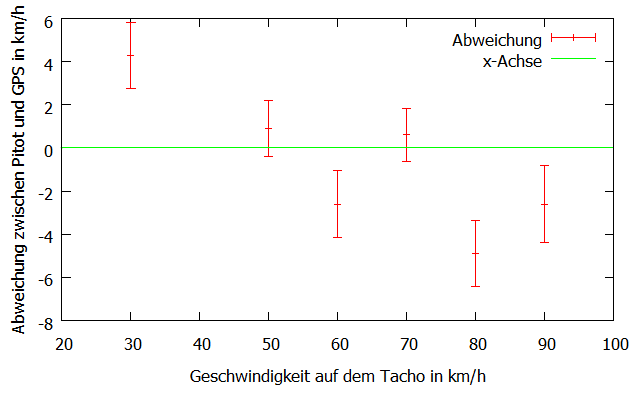
\includegraphics[width=.9\textwidth]{images/AbweichungGPSPitot}
\caption{Abweichung der mit dem Pitotrohr und mit GPS gemessenen Geschwindigkeit}
\label{fig:AbweichungGPSPitot}
\end{figure}
\\
\\
In Abbildung \ref{fig:AbweichungGPSPitot} ist die Differenz zwischen der mit dem Pitotrohr und mit GPS gemessenen Geschwindigkeit dargestellt. Man sieht:
\begin{enumerate}
\item Die Abweichungen liegen im Bereich von -6 bis +6 km/h, insbesondere gibt es sowohl positive wie auch negative Abweichungen, wobei der Fehler wie vorhin erklärt zu klein ist.
\item Für 80 und 90 km/h ergeben sich große negative Abweichungen. Möglicherweise ist hier aufgrund der hohen Strömungsgeschwindigkeit die Strömung auf dem Autodach nicht mehr laminar, bzw. es entstehen unvorhersehbare Turbulenzen.
\item Die Abweichungen sind sowohl im Betrag als auch im Vorzeichen unterschiedlich und folgen keiner erkennbaren Verteilung. Eine mögliche Erklärung ist, dass die Strömungsgeschwindigkeit auf dem Autodach natürlich vom Wind beeinflusst wird. Je nach Windrichtung wird dann das Ergebnis größer oder kleiner.
\end{enumerate}

\section{Fazit}
Insgesamt lässt sich sagen, dass die Messung trotz des simplen Aufbaus und der einfachen Konstruktion des Pitotrohrs gut funktioniert und erstaunlich genaue Ergebnisse geliefert hat. Als Geschwindigkeitsmesser für das Auto oder andere Fahrzeuge eignet sich das Pitotrohr aber doch nur bedingt, insbesondere da die Messergebnisse durch den Wind verfälscht werden können. Der Tachometer hat den klaren Vorteil, auch gegenüber dem eigentlich genaueren GPS, dass seine Anzeige quasi nicht von äußeren Einflüssen abhängt und damit zwar keine genauen, aber immer zuverlässige Werte liefert. Für die Messung von Strömungsgeschwindigkeiten, die z.B. bei Flugzeugen oder auch Rennwagen für die Aerodynamik entscheidend sind, ist es aber ideal geeignet. Es ist zu erwarten, dass mit professionell gebauten Systemen sehr gute Messgenauigkeiten erreicht werden können.